\documentclass[12pt, oneside]{article}
\usepackage[letterpaper, margin=1in]{geometry}
\usepackage[english]{babel}
\usepackage[utf8]{inputenc}
\usepackage{amsmath}
\usepackage{amsfonts}
\usepackage{amssymb}
\usepackage{tikz}

\usepackage{fancyhdr}
\pagestyle{fancy}
\fancyhf{}
\rhead{Name: \hspace{1.5in} }
\lhead{BECA / Dr. Huson / Algebra 2 \\* 11 January 2018 \\* Test: Exponents and exponential functions}

\renewcommand{\headrulewidth}{0pt}

\title{Worksheet and test template}
\author{Chris Huson}
\date{January 2018}

\begin{document}

\subsubsection*{\\* Simplify expressions}

Simplify by collecting like terms.

\begin{enumerate}

\item $-2x^2+4x -19 +12x^2-4x+9$\\*[60pt]
\item $-2(a^2-3a +6) -3(a^2-2a-4)$\\*[60pt]

\subsubsection*{Solve equations}

Solve for the value of $x$.
\item   $16=-x-3x$\\*[50pt]
\item   $\frac{1}{3}(30-27x)=x$\\*[60pt]
\item   $10=\frac{1}{4}x+2.75x-8$\\*[60pt]

\newpage
\subsubsection*{Slope-intercept form}

What is the slope and $y$-intercept of each equation? 
\item   $y=\frac{1}{3}x-4.2$\\*[10pt]
\item   $x+2y=6$\\*[40pt]


\subsubsection*{Parallel and perpendicular linear equations}

\item What is the equation of the line with a slope of 2 passing through the point $(0,-5)$?\\*[40pt]
\item What is the equation of a line parallel to $y=-2x+6$ with a $y$-intercept of 3?\\*[40pt]
\item What is the slope of a line perpendicular to the line $3x+12y=11$?\\*[50pt]

\subsubsection*{Function substitution}
\item Given $f(x)=4x-13$. Simplify $f(\frac{3}{2})$.\\*[50pt]
\item Given $\displaystyle f(x)=\frac{(11-x)}{5x}$. Simplify $f(-1)$.

\newpage
\subsubsection*{Graphing linear functions}
Use pencil for graphs. Label each function with its name or equation. 
\item Given the function $f(x)=-\frac{1}{2}x+4$. 
\begin{enumerate}
    \item Write down the $y$-intercept.\\*[10pt]
    \item Write down the slope of $f(x)$.\\*[10pt]
    \item Draw the function $f(x)$ on the graph below.
    \item Mark and label the point $Q (4, -2)$ on the graph.
    \item A second line, $g(x)$, is parallel to $f(x)$ and passes through point $Q$. Plot $g(x)$ on the graph.
    \item What is the $y$-intercept of $g(x)$?\\*[10pt]
\end{enumerate}

\begin{figure}[!ht]
    \centering
    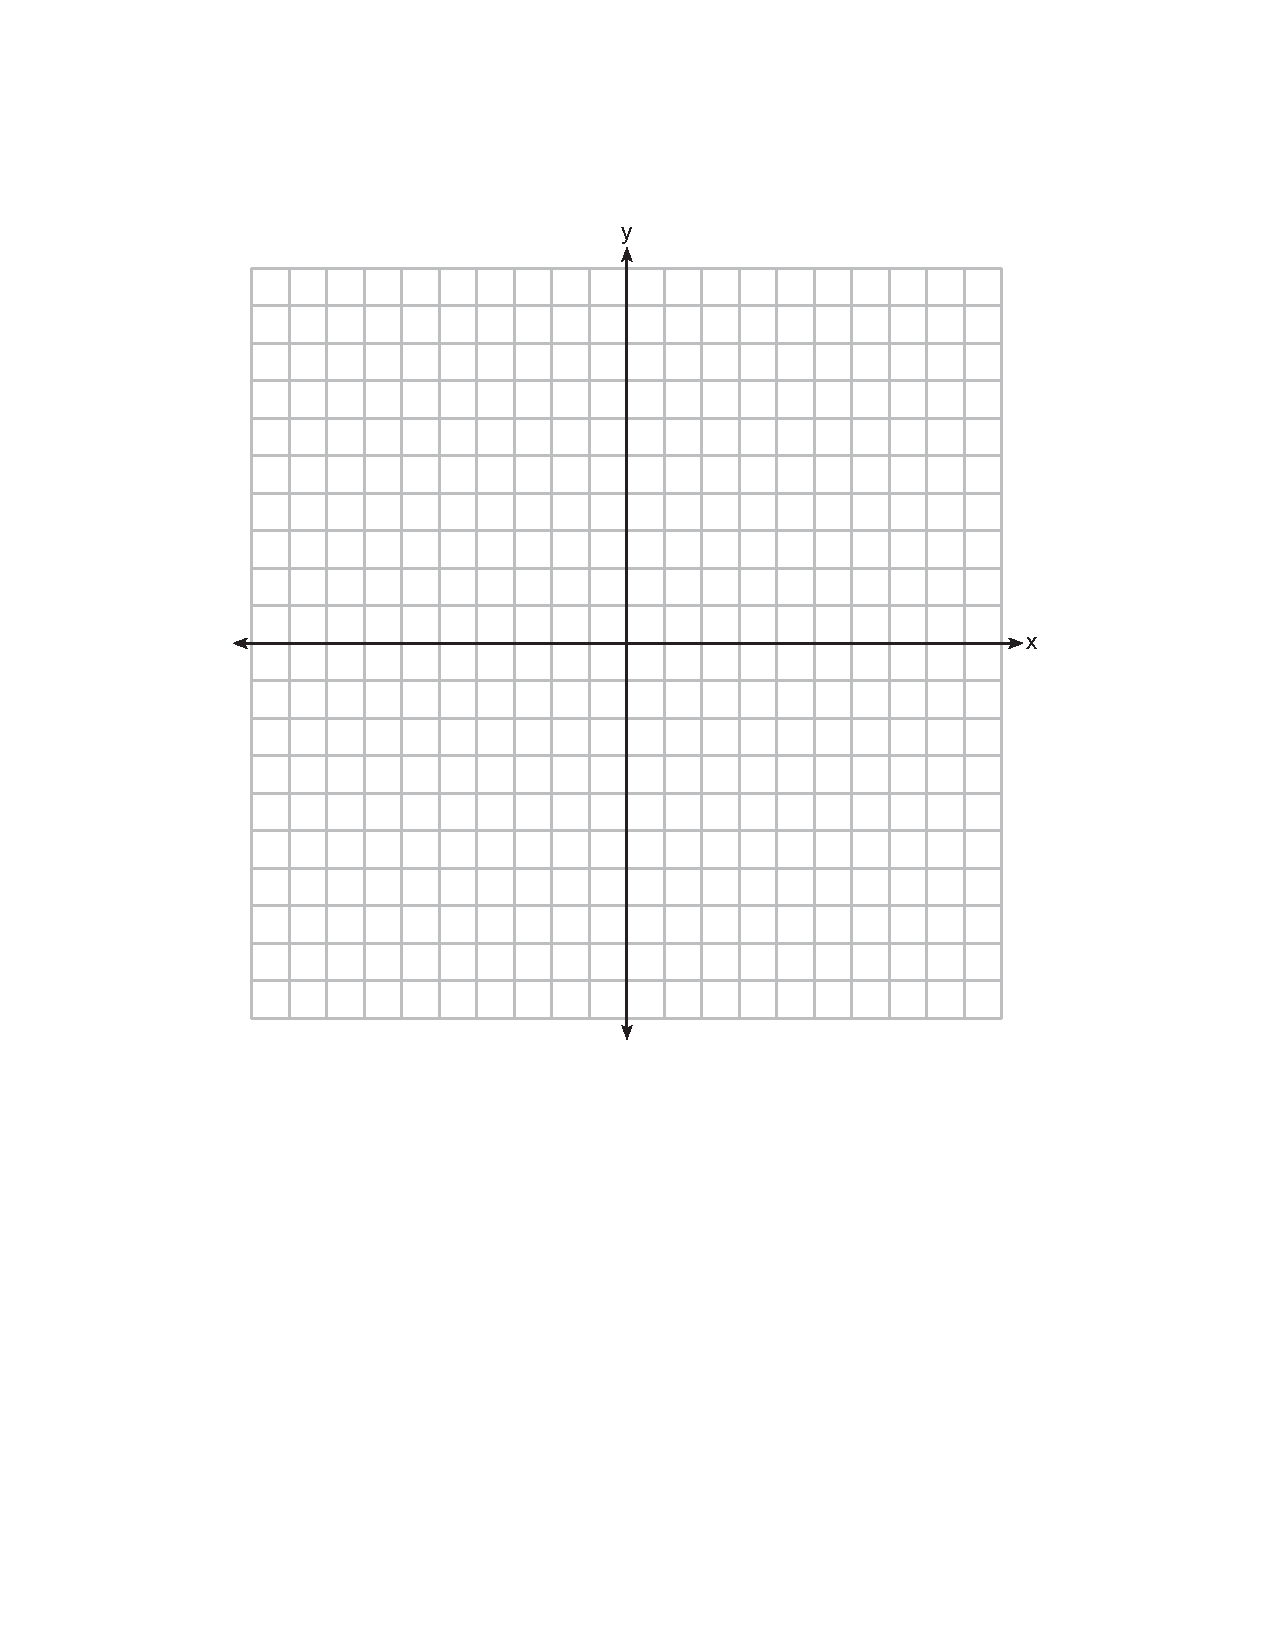
\includegraphics[width=0.75\textwidth]{regents-grid.pdf}
\end{figure}

\newpage
\item  
\begin{enumerate}
    \item On the axes below, for $-3 \leq x \leq 5$, graph $f(x)=2^{x-1}-8$

    \item What is the $y$-intercept of the function?\\*[20pt]
    \item The function $f$ has an asymptote. Draw the asymptote.
    \item What is the equation of the asymptote?\\*[20pt]

    \item On the graph, mark and label the point $P (2, f(2))$.

\begin{figure}[!ht]
    \centering
    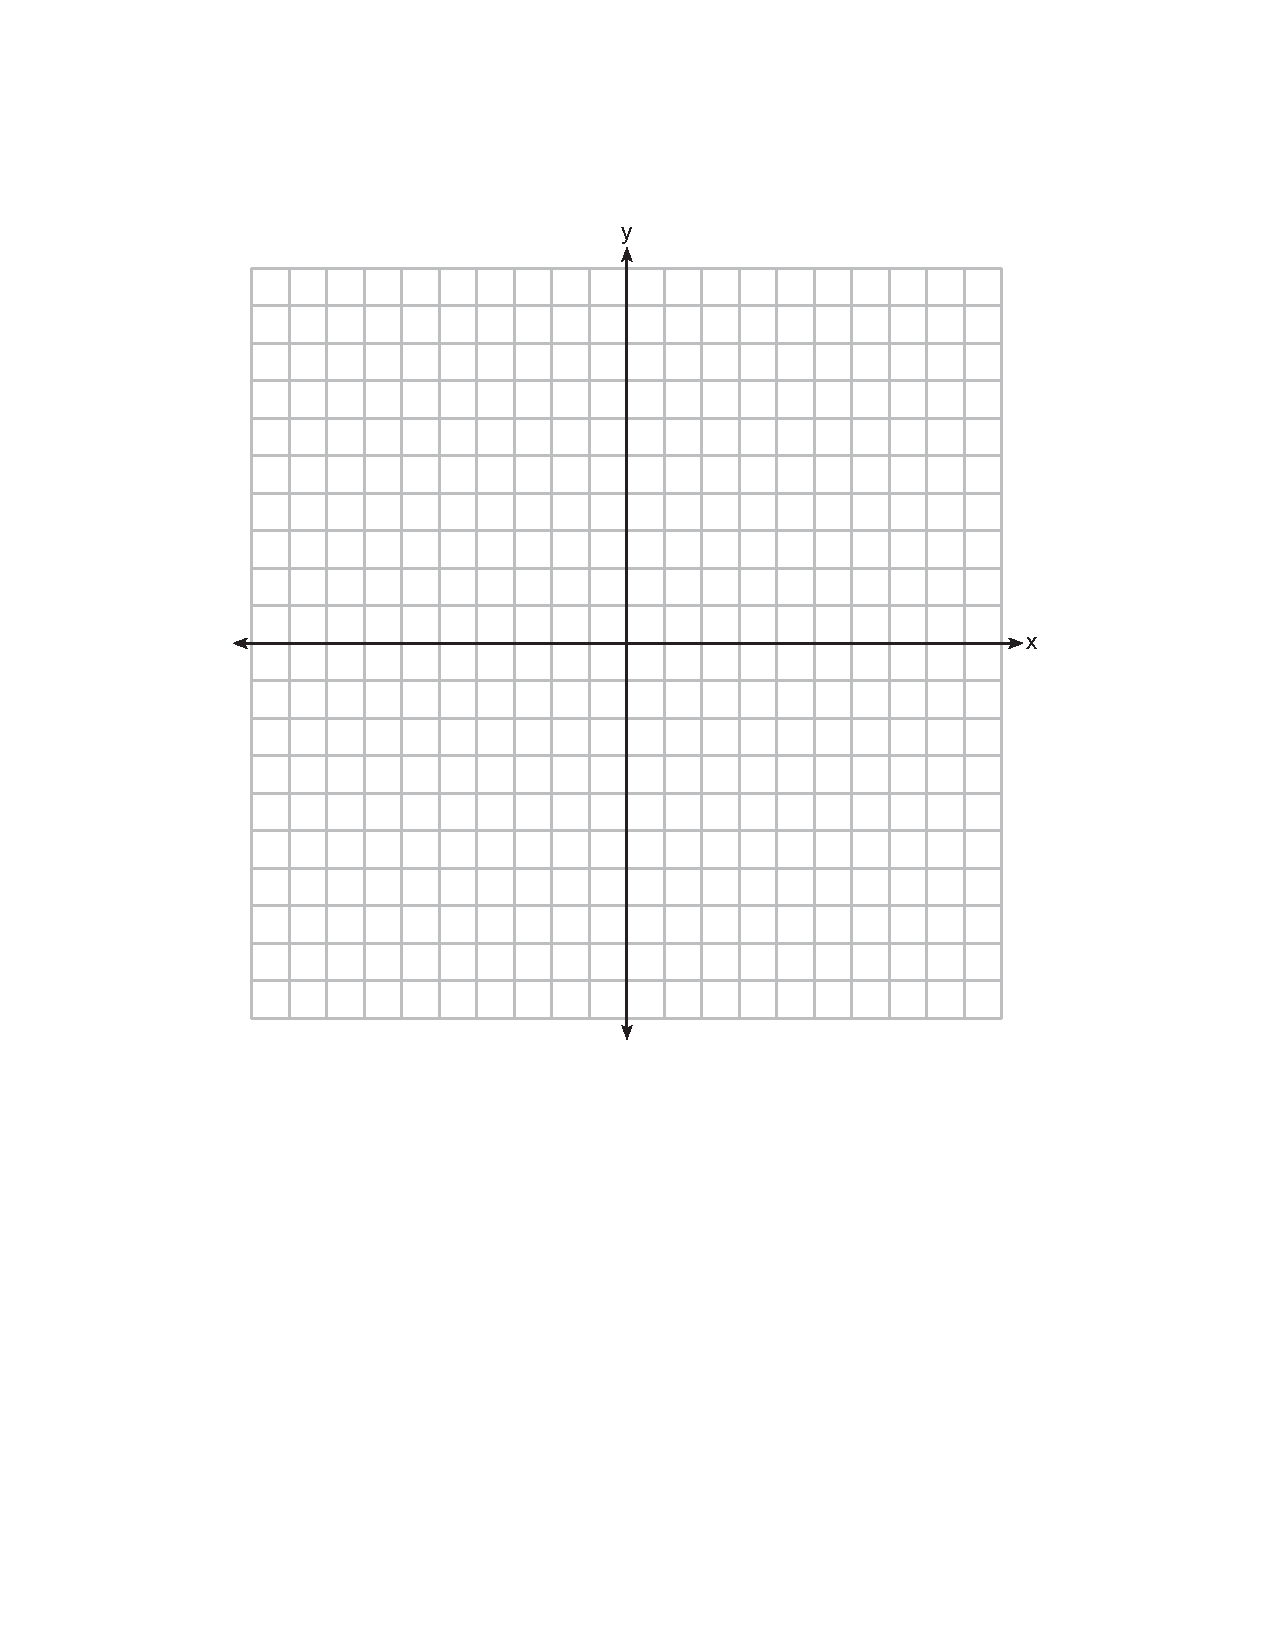
\includegraphics[width=0.65\textwidth]{regents-grid.pdf}
\end{figure}
\end{enumerate}

\item Explain why the radical $\sqrt[3]{49}$ is equivalent to $7^{\frac{2}{3}}$, an expression with a rational exponent.

\newpage
\item Solve the system of equations by graphing. Select a point in the solution set and label it on the graph as ordered pair.
\[x+y \geq 5\]
\[-2x+y > -4\]

\begin{figure}[!ht]
    \centering
    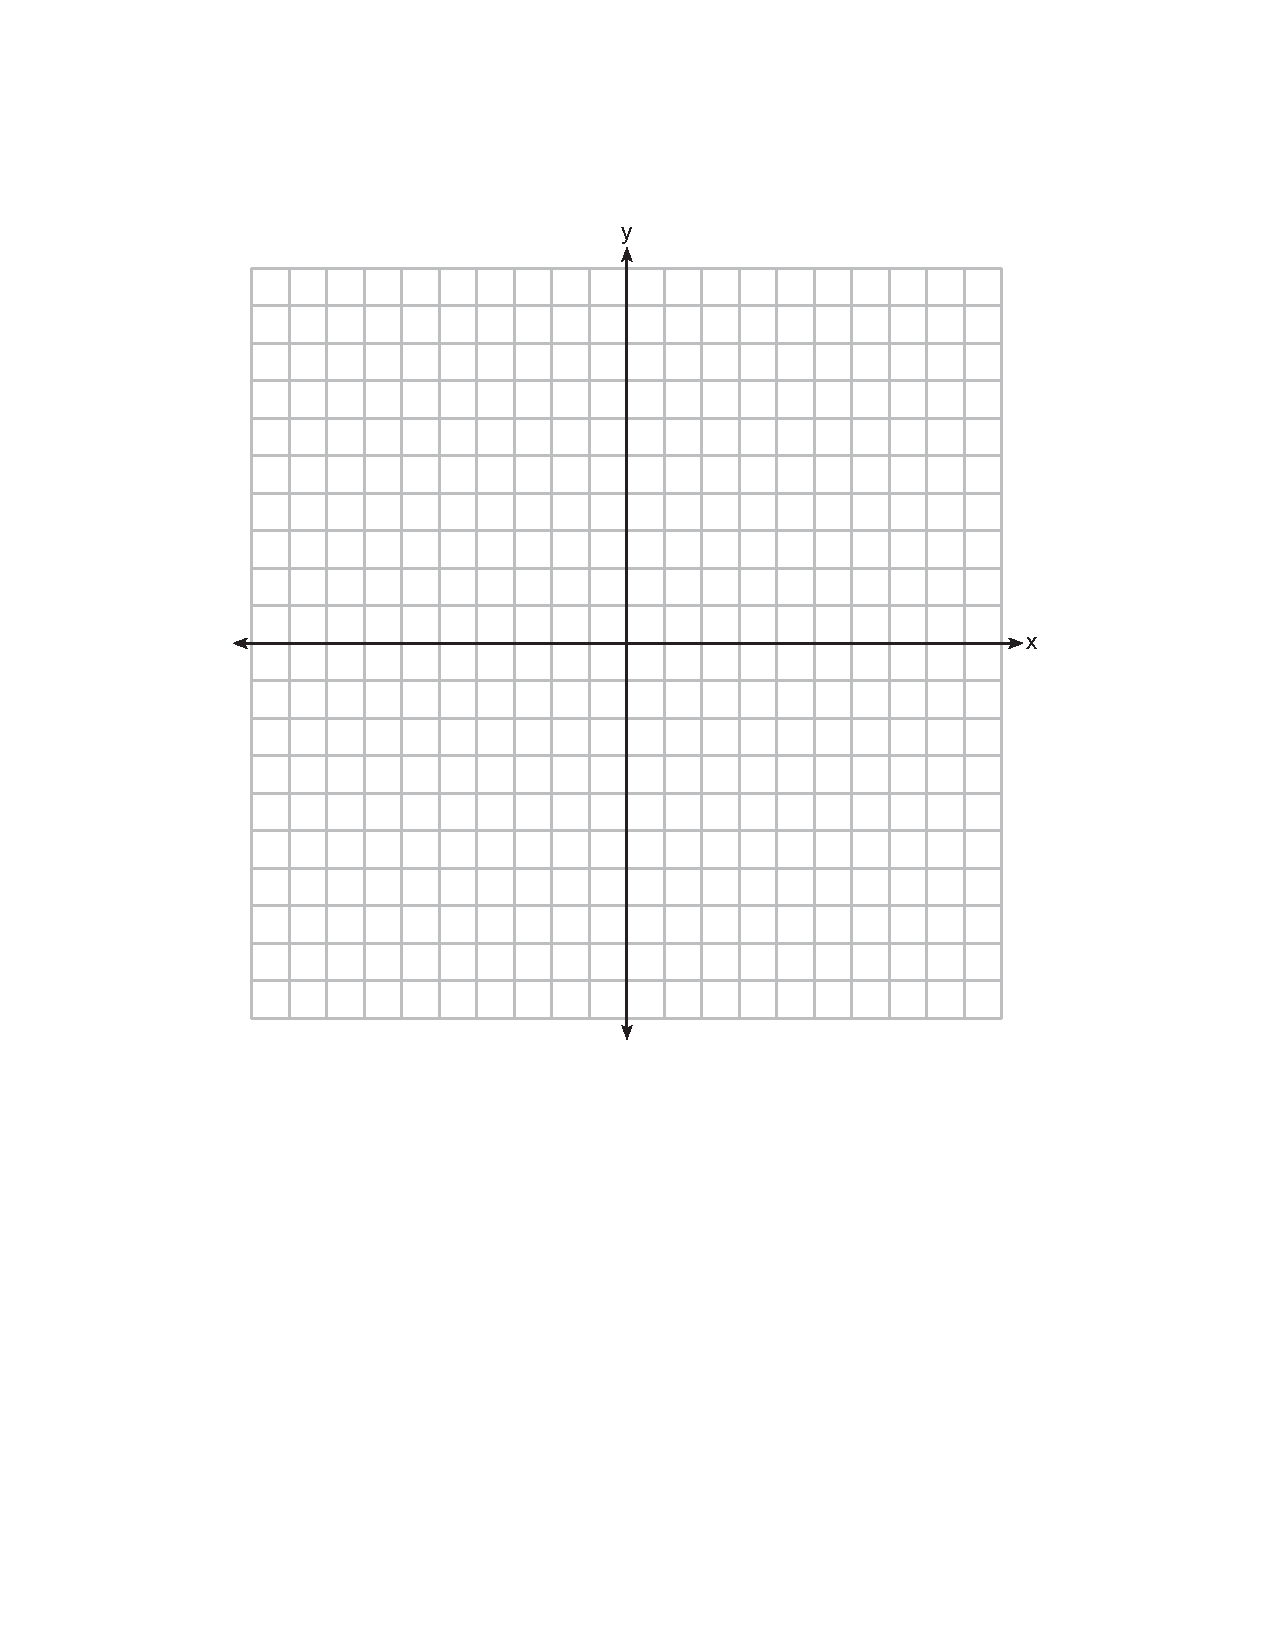
\includegraphics[width=0.65\textwidth]{regents-grid.pdf}
\end{figure}

Solve the system algebraically.
\item
$-x+4y=-6$\\*
$5x-18y=28$\\*[60pt]

\item 
$y=log_5{25}$\\*
$y=3^x-7$

\newpage
\item Oceanside Bike Rental Shop charges a 11.50 dollar bike fee plus 3.25 dollars an hour for renting a bike. Jeffrey paid 21.25 dollars total. How many hours did he pay to have the bike checked out? (write an equation first, then solve it)\\*[160pt]

\item Seth's parents gave him \$5000 to invest for his 16th birthday. He is considering two investment
options. Option A will pay him 4.5\% interest compounded annually. Option B will pay him 4.6\%
compounded quarterly.
\begin{enumerate}
    \item Write a function of option A and option B that calculates the value of each account after n years.\\*[95pt]
    \item Seth plans to use the money after he graduates from college in 5 years. Determine how much money option A will earn, to the nearest cent.
\end{enumerate}

\end{enumerate}
\end{document}